\documentclass{beamer}

\usepackage[T1]{fontenc}
\usepackage{graphicx}
\usepackage{tikz}
\usepackage{booktabs}
\usepackage{minted}
\usepackage{hyperref}
\usepackage[dvipsnames]{xcolor}
\usepackage[spanish]{babel}

\usetikzlibrary{shapes.geometric, arrows.meta, positioning}
\tikzstyle{startstop} = [rectangle, rounded corners, minimum width=3cm, minimum height=1cm,text centered, draw=black, fill=blue!20]
\tikzstyle{process} = [rectangle, minimum width=3.2cm, minimum height=1cm, text centered, draw=black, fill=gray!10]
\tikzstyle{io} = [trapezium, trapezium left angle=70, trapezium right angle=110, minimum width=3.2cm, minimum height=1cm, text centered, draw=black, fill=orange!20]
\tikzstyle{arrow} = [thick, ->, >=stealth]
\usemintedstyle{manni}

\usetheme{Berlin}
\setbeamercolor{structure}{fg=RoyalPurple}

\title[Motor y editor de videojuegos en 2D enfocado al desarrollo de juegos RPG]{Motor y editor de videojuegos en 2D enfocado al desarrollo de juegos RPG}
\subtitle{2D video game engine and editor focused on RPG game development}
\author[Miguel Curros, Alejandro González y Alejandro Massó]{Miguel Curros García\\ Alejandro González Sánchez\\ Alejandro Massó Martínez}
\date{10 de junio de 2025}

\newcommand{\baker}{%
	\textsc{RPGBaker}%
}

\newcommand{\comillas}[1]{\guillemotleft #1\guillemotright{}}

\begin{document}

\frame{\titlepage}

\begin{frame}{Índice}
	\tableofcontents
\end{frame}

\section{Objetivos}
\begin{frame}{Objetivos (I)}
a
\end{frame}

\section{Planteamiento}
\begin{frame}{Planteamiento (I)}
a
\end{frame}
\section{Diseño del motor de \baker}
\begin{frame}{Diseño del motor (I) }
a
\end{frame}

\section{Diseño del editor de \baker}
\begin{frame}{Editor de \baker}
	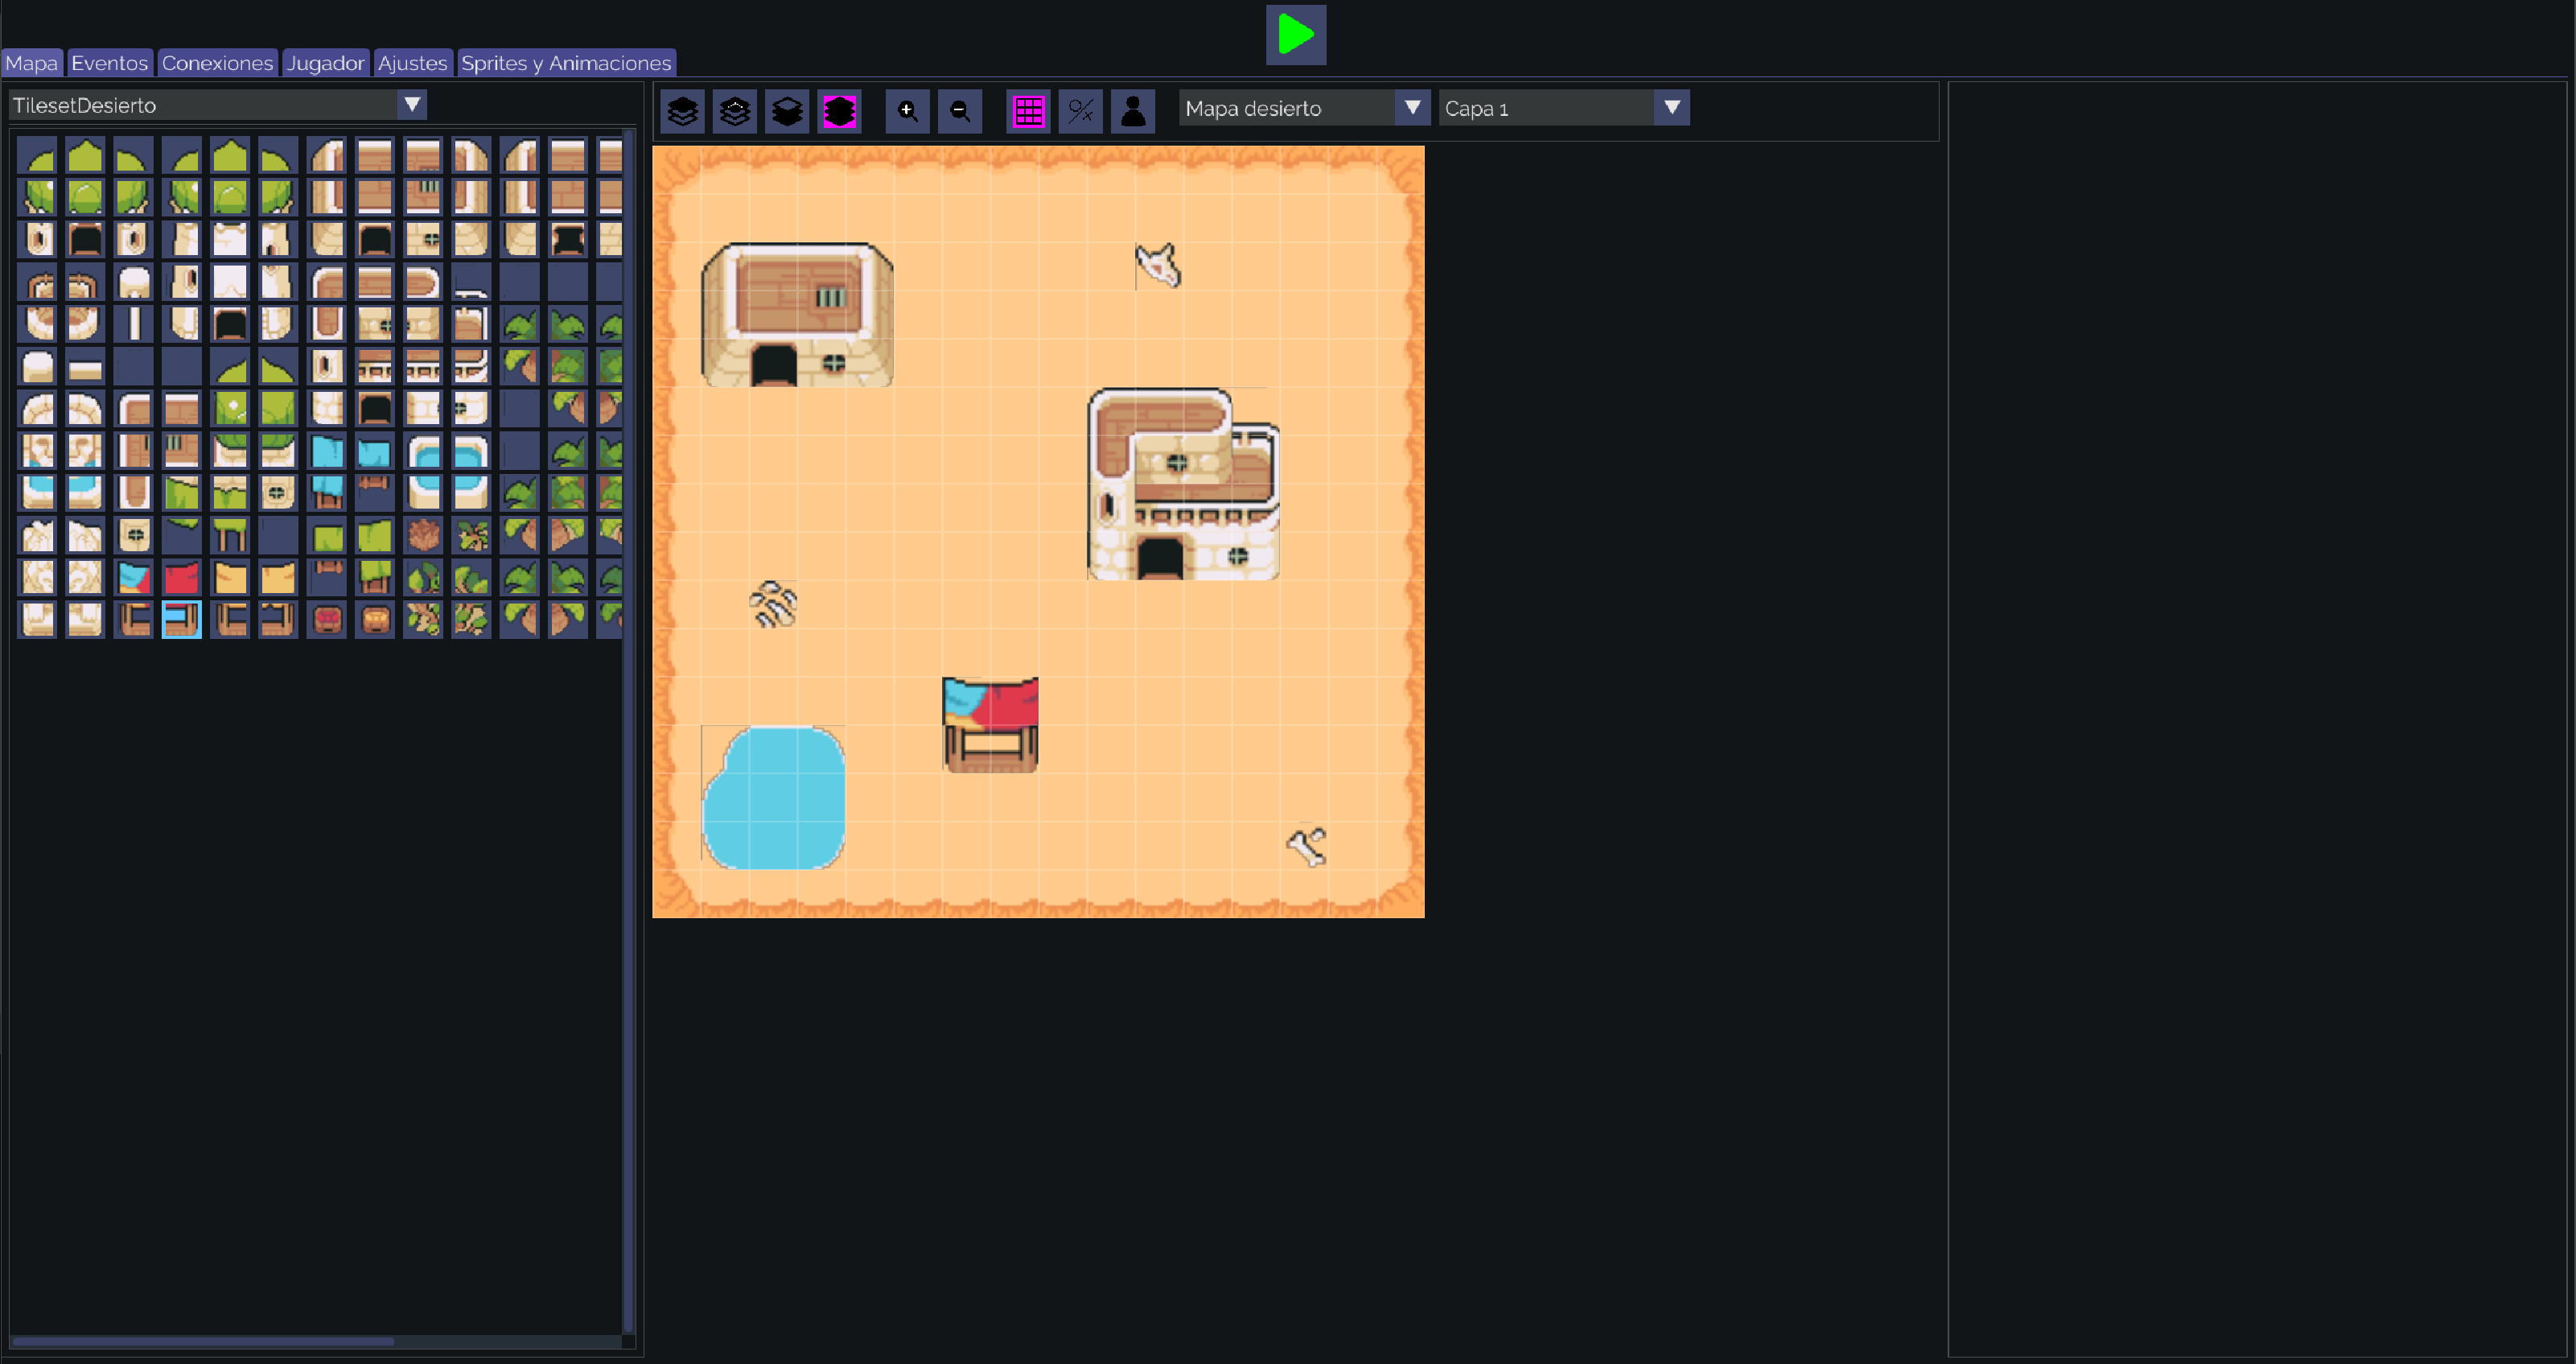
\includegraphics[width=\textwidth]{imgs/editor/editorMapas.pdf}
\end{frame}

\begin{frame}{Funcionalidades principales}
	\begin{columns}
		\column{0.4\textwidth}
			\begin{itemize}
				\item Edición de mapas de manera interactiva.
				\item Gestión de recursos gráficos, como \textit{sprites} o animaciones.
				\item Edición de eventos con condiciones y comportamientos personalizables.
				\item Carga y guardado de proyectos con persistencia completa.
			\end{itemize}
		\column{0.6\textwidth}
			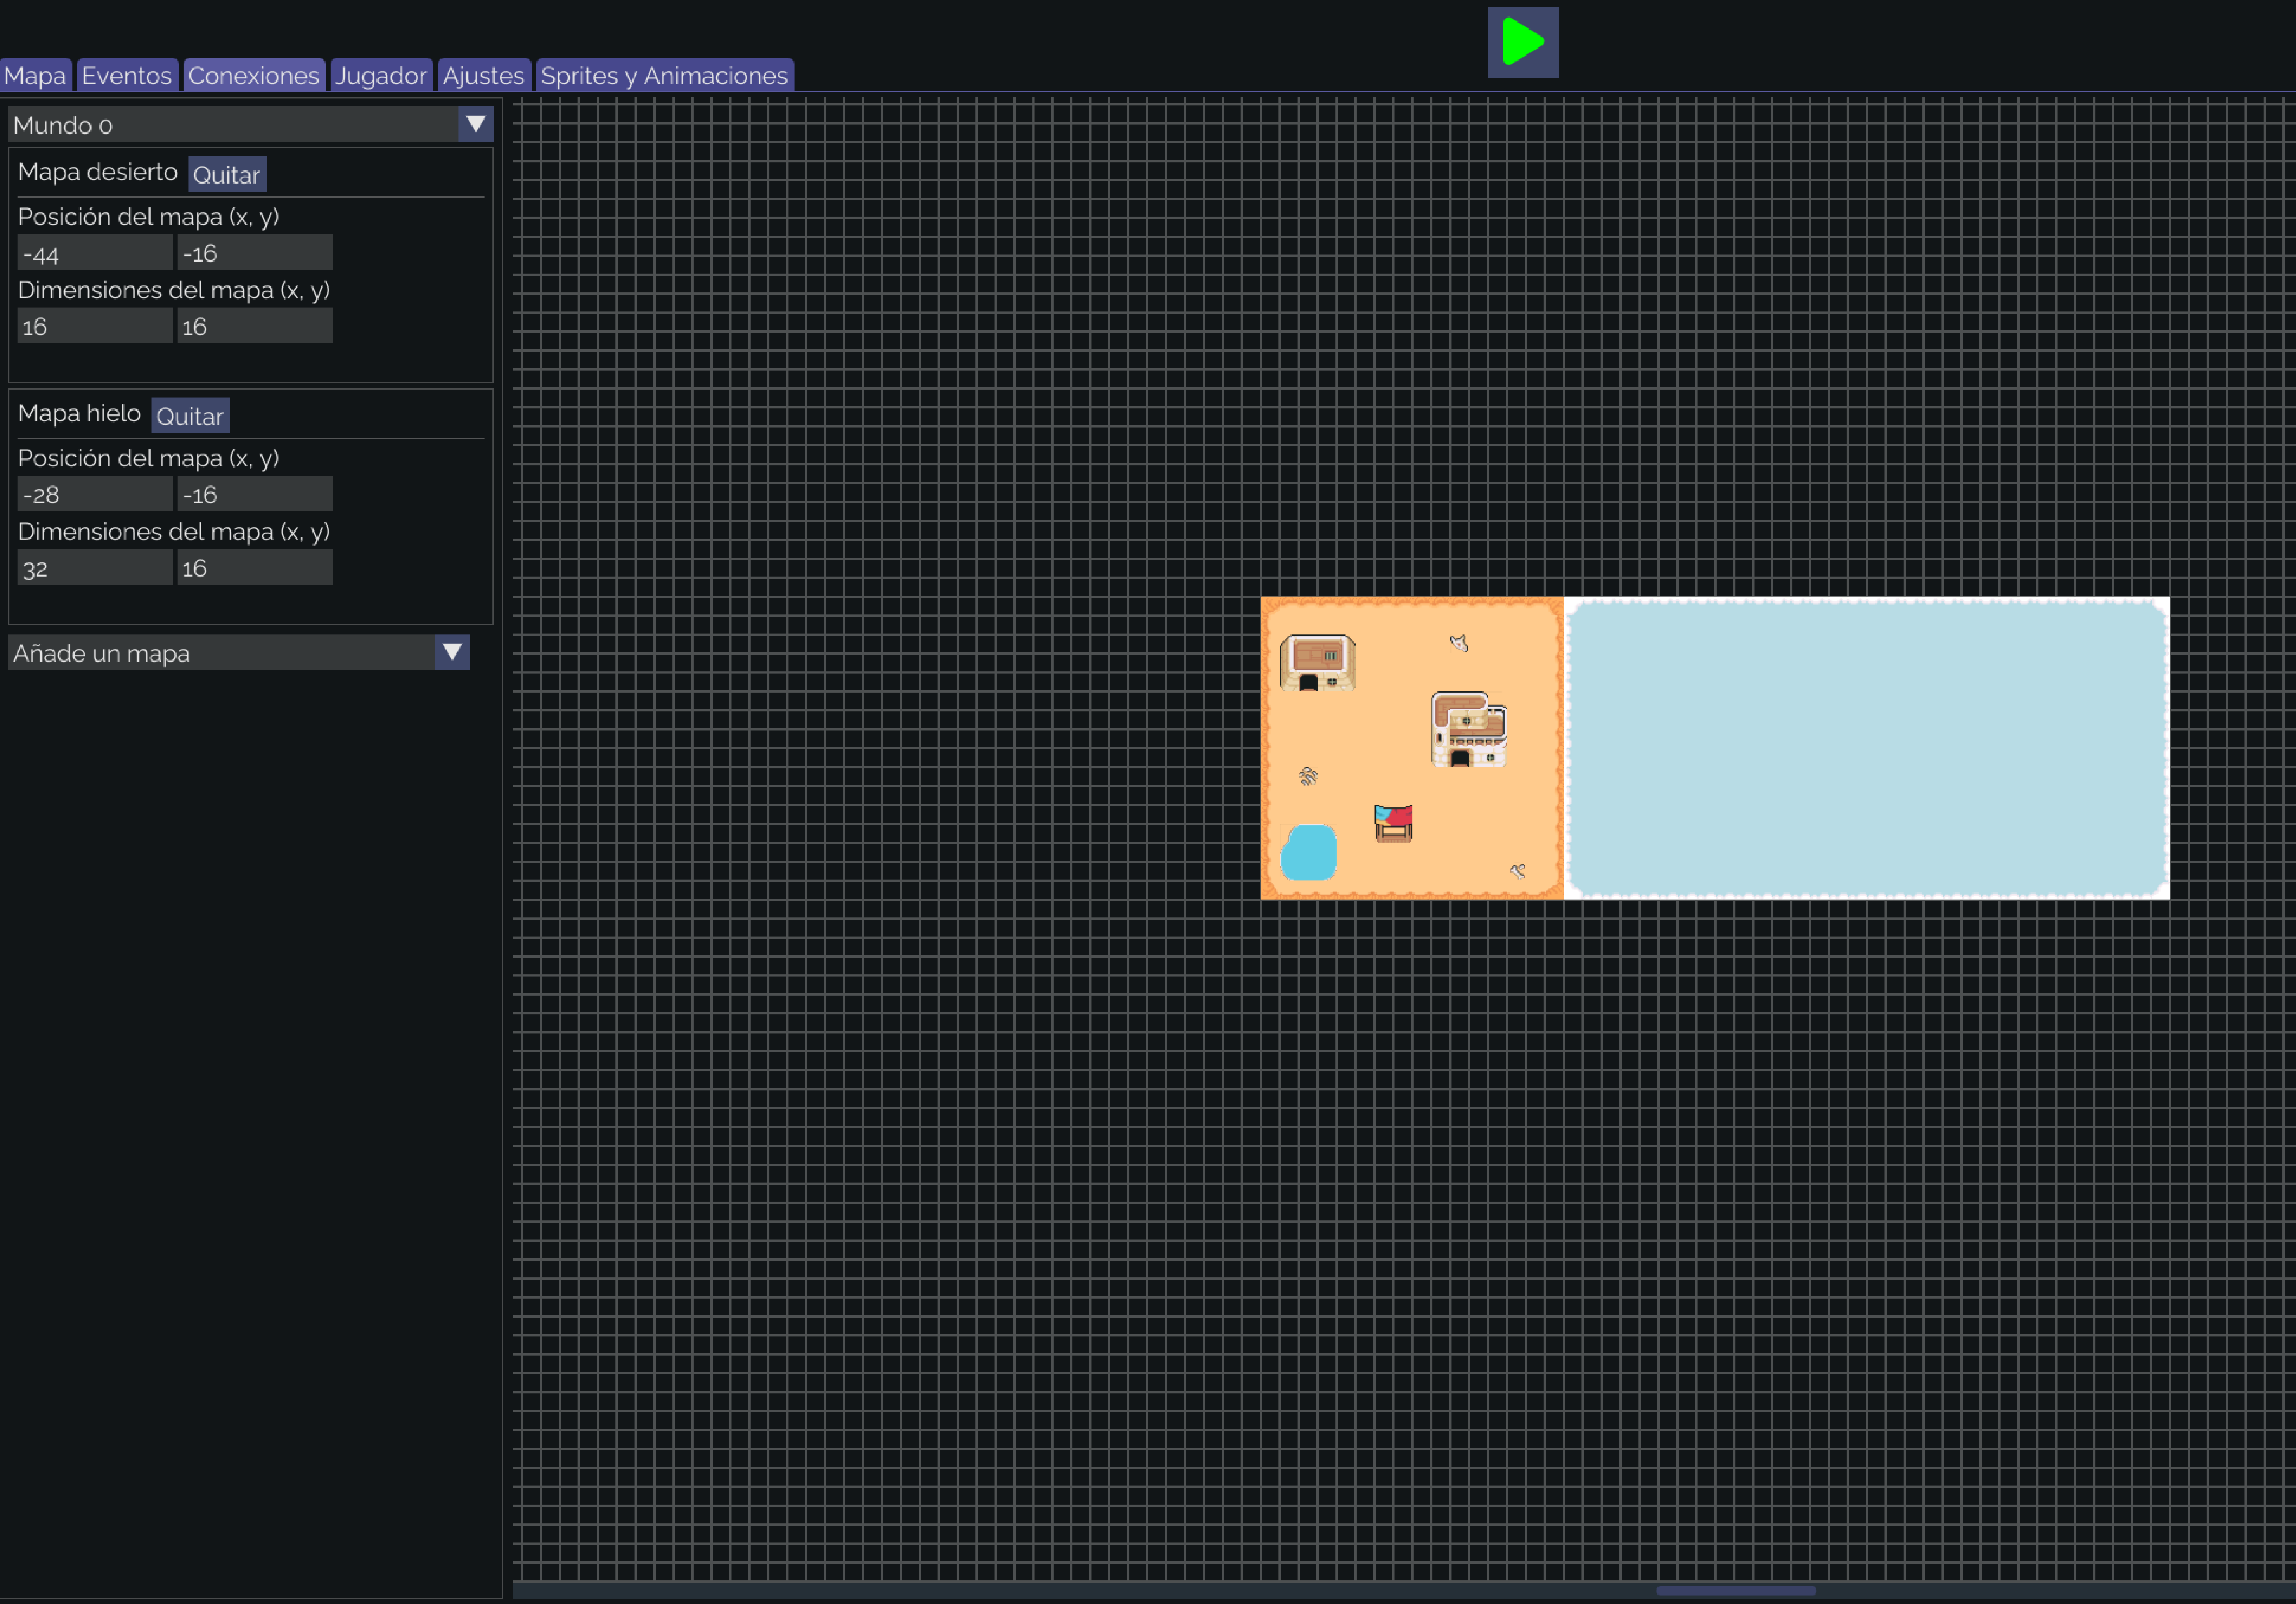
\includegraphics[width=\textwidth]{imgs/editor/conexiones.pdf}
	\end{columns}
\end{frame}

\begin{frame}{Interfaz y usabilidad}
	\begin{columns}
		 \column{0.4\textwidth}
		 	\begin{itemize}
		 		\item Interfaz basada en ventanas y pestañas: clara, modular y adaptable.
		 		\item Pensada para usuarios novatos.
		 		\item Pestañas dependiendo de su función: editor de mapas, de eventos, de recursos\ldots
		 		\item Soporte de elementos visuales como \textit{tooltips} o mensajes de error.
		 	\end{itemize}
		 \column{0.6\textwidth}
		 	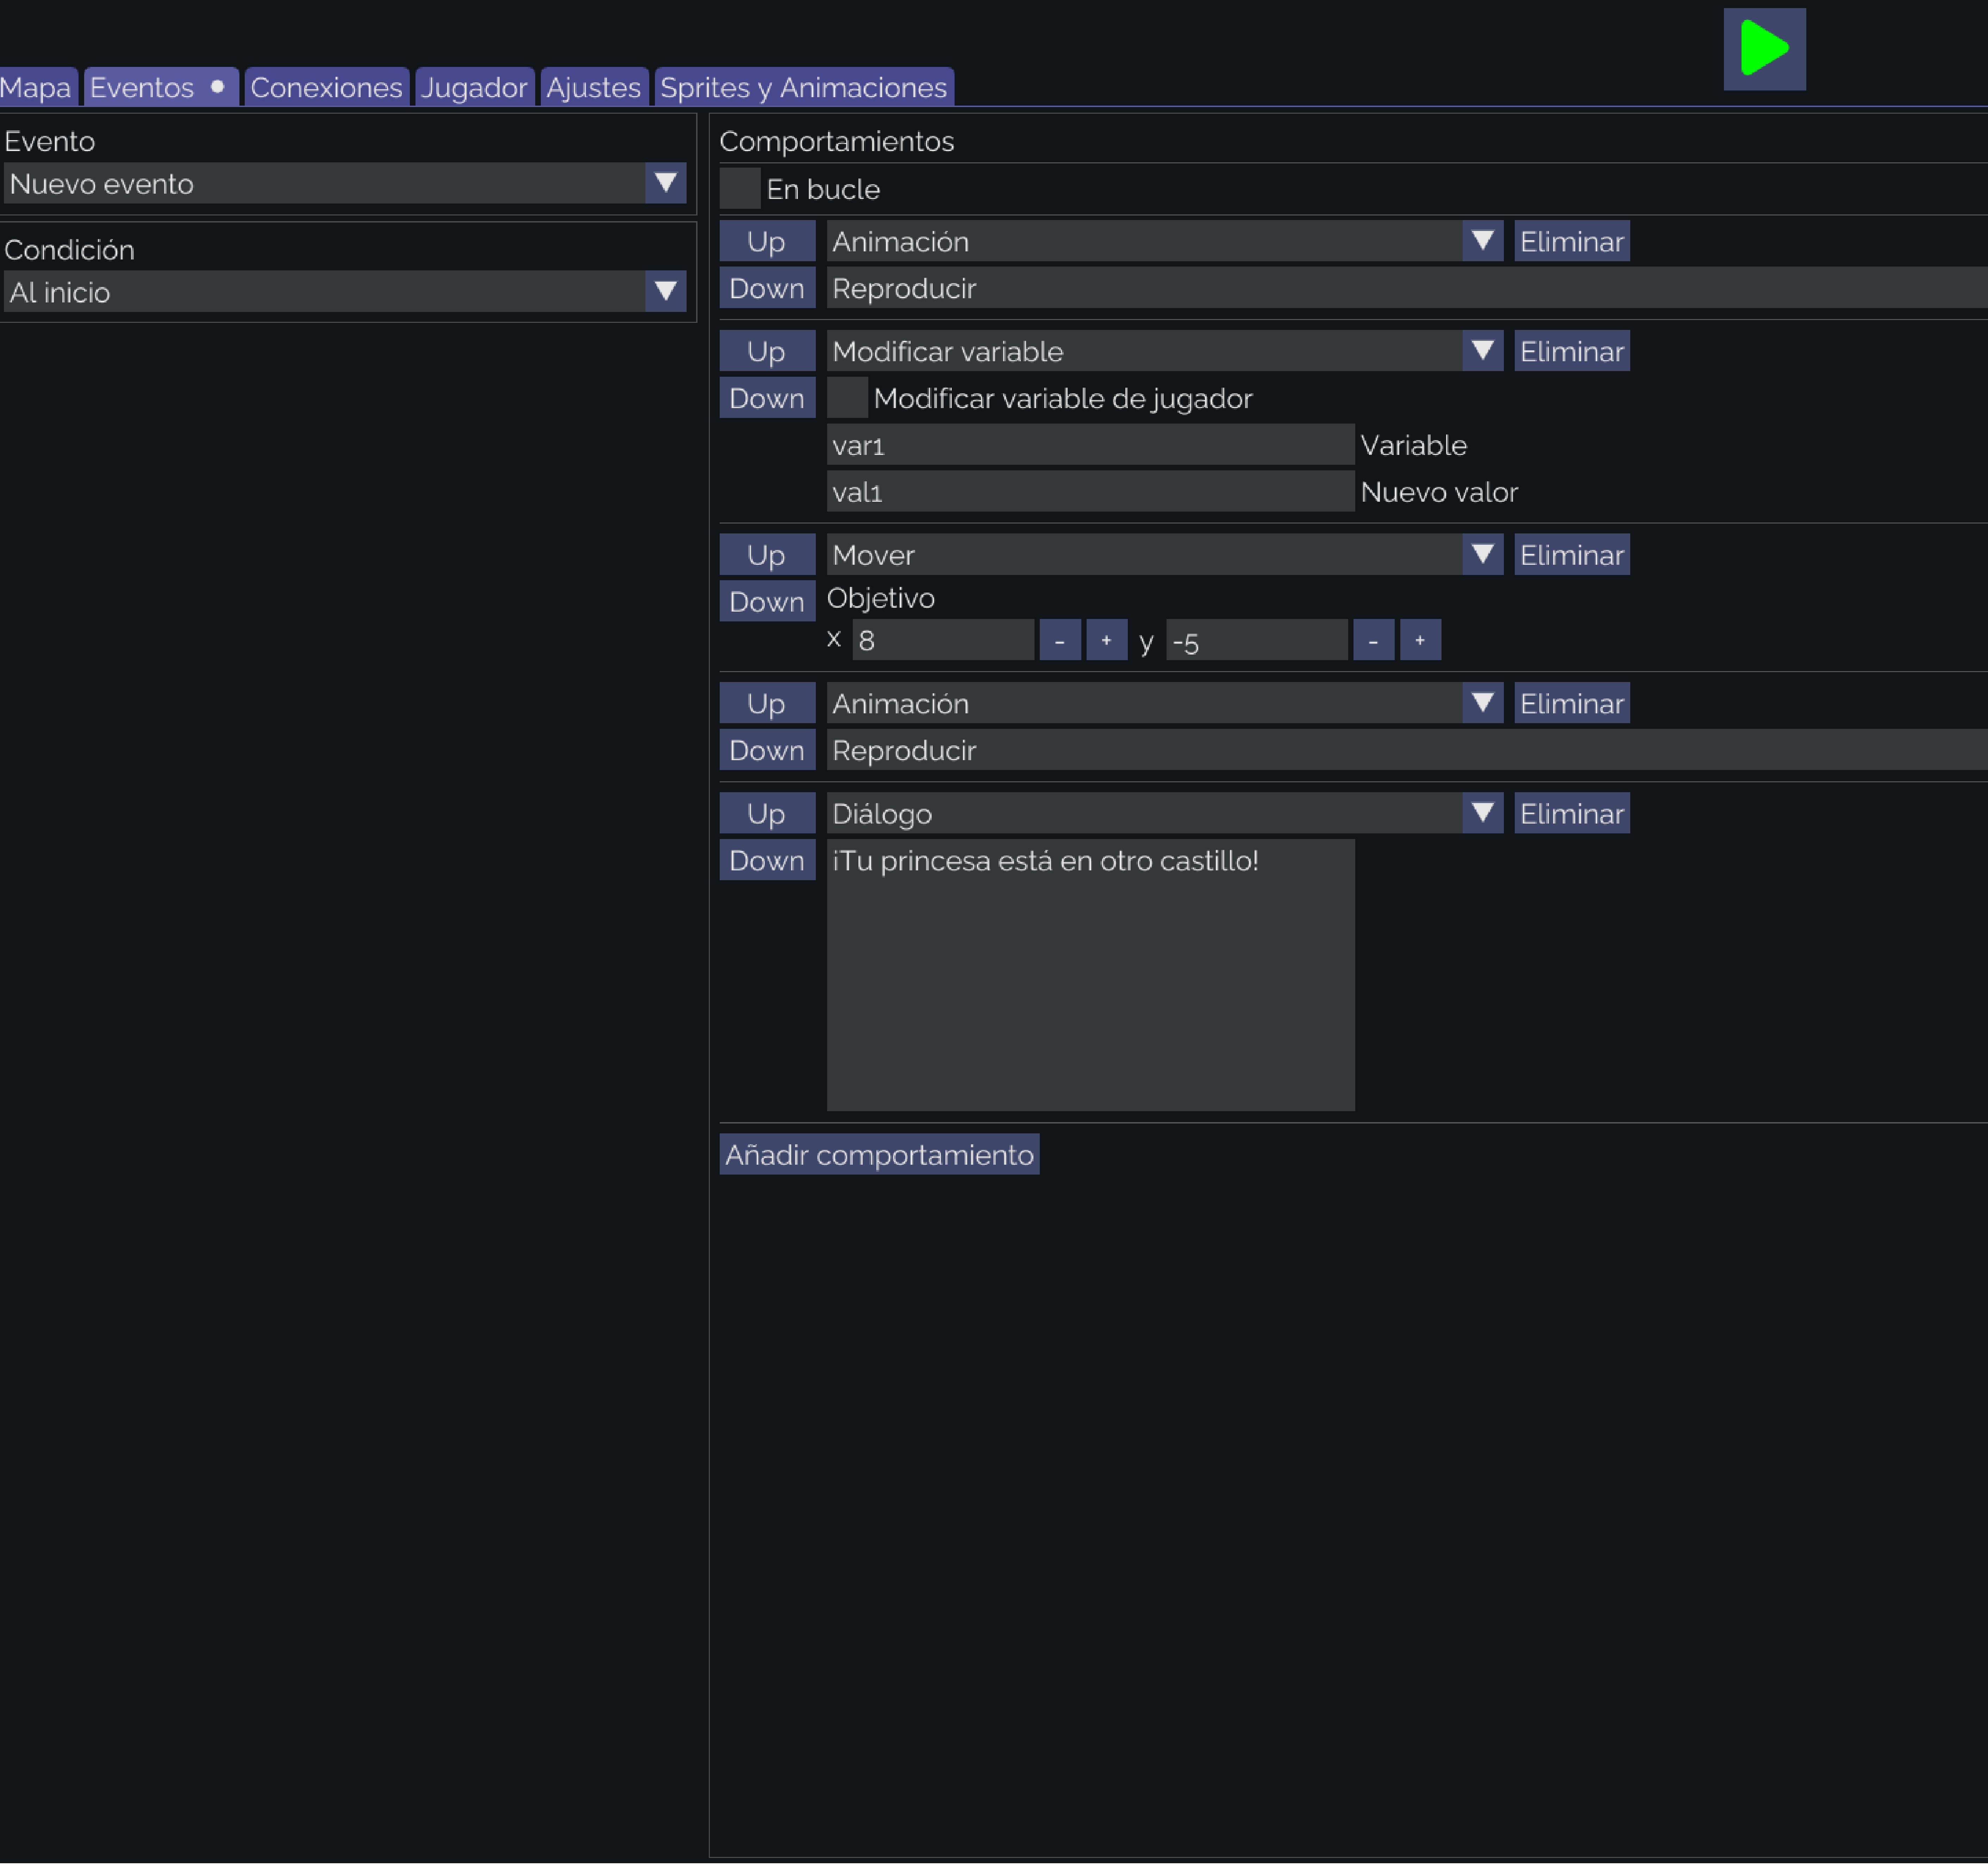
\includegraphics[width=\textwidth]{imgs/editor/eventos.pdf}
	\end{columns}
\end{frame}

\begin{frame}{\textit{Build} multiplataforma al motor}
	\begin{columns}
		 \column{0.4\textwidth}
		 	\begin{itemize}
		 		\item Se generan ejecutables para Windows, MacOS, Linux y Android.
		 		\item No requiere de recompilación manual ni de pasos adicionales.
		 		\item El editor \comillas{traduce} sus datos a la sintaxis esperada por el motor.
		 	\end{itemize}
		 \column{0.6\textwidth}
		 	\begin{center}
		 	\scalebox{0.5}{
		 	\begin{tikzpicture}[node distance=1.5cm and 2cm]
		 		\node (start) [startstop] {Usuario diseña el juego en el editor};
		 		\node (data) [process, below=of start] {Datos del proyecto};
				\node (convert) [process, below=of data] {Serialización y empaquetado};
				\node (build) [process, below=of convert] {Generación del ejecutable};
				\node (win) [io, below left=1.5cm and 2.5cm of build] {Windows};
				\node (mac) [io, below left=1.5cm and -1.0cm of build] {MacOS};
				\node (linux) [io, below right=1.5cm and -1.0cm of build] {Linux};
				\node (andr) [io, below right=1.5cm and 2.5cm of build] {Android};
				
				\draw [arrow] (start) -- (data);
				\draw [arrow] (data) -- (convert);
				\draw [arrow] (convert) -- (build);
				\draw [arrow] (build) -- (win);
				\draw [arrow] (build) -- (mac);
				\draw [arrow] (build) -- (linux);
				\draw [arrow] (build) -- (andr);
		 	\end{tikzpicture}
		 	}
		 	\end{center}
	\end{columns}
\end{frame}

\title[2D video game engine and editor focused on RPG game development]{Motor y editor de videojuegos en 2D enfocado al desarrollo de juegos RPG}
\author[Miguel Curros, Alejandro González and Alejandro Massó]{Miguel Curros García\\ Alejandro González Sánchez\\ Alejandro Massó Martínez}

\section{Contributions}
\begin{frame}{Miguel Curros García}
a
\end{frame}

\begin{frame}{Alejandro González Sánchez}
a
\end{frame}

\begin{frame}{Alejandro Massó Martínez}
	\begin{itemize}
		\item Research on general and specific RPG editors.
		\item \baker{}'s editor design.
		\item Project's toolchain development.
		\item \baker{}'s editor development.
		\item Report writing.
	\end{itemize}
\end{frame}

\end{document}